\documentclass[12pt, a4paper]{report}

\usepackage[a4paper, top=3cm, bottom=3cm, left=4cm, right=3cm]{geometry}
\usepackage{setspace}
\onehalfspacing

% Typography & Language
\usepackage[utf8]{inputenc}
\usepackage[T1]{fontenc}
\usepackage{lmodern}
\usepackage[indonesian]{babel}
\usepackage{microtype}
\usepackage{xurl}

% Typography penalties & spacing hygiene
\clubpenalty=10000
\widowpenalty=10000
\displaywidowpenalty=10000
\emergencystretch=2.5em
\raggedbottom

% Prevent hyphenation in headings
\usepackage{titlesec}
\titleformat{\chapter}[display]{\normalfont\huge\bfseries\raggedright}{\chaptertitlename\ \thechapter}{20pt}{\Huge}
\titleformat{\section}{\Large\bfseries\raggedright}{\thesection}{1em}{}
\titleformat{\subsection}{\large\bfseries\raggedright}{\thesubsection}{1em}{}
\titleformat{\subsubsection}{\normalsize\bfseries\raggedright}{\thesubsubsection}{1em}{}

% Math & Symbols
\usepackage{amsmath, amssymb, amsfonts}

% Tables & Figures
\usepackage{graphicx}
\usepackage{booktabs}
\usepackage{tabularx}
\usepackage{xltabular}
\usepackage{multirow}
\usepackage{caption}
\usepackage{subcaption}
\usepackage{float}
\usepackage{enumitem}
\setlist{noitemsep, topsep=3pt, parsep=1pt, partopsep=0pt}

% TikZ for crisp diagrams
\usepackage{tikz}
\usetikzlibrary{shapes.geometric, arrows.meta, positioning, fit, backgrounds, calc}

% Colors & Code Listings
\usepackage{xcolor}
\definecolor{codegreen}{rgb}{0,0.6,0}
\definecolor{codegray}{rgb}{0.45,0.45,0.45}
\definecolor{codepurple}{rgb}{0.58,0,0.82}
\definecolor{backcolour}{rgb}{0.97,0.97,0.97}
\definecolor{itbblue}{rgb}{0.0,0.2,0.5}
\definecolor{boxbg}{rgb}{0.93,0.95,0.99}
\definecolor{boxborder}{rgb}{0.2,0.4,0.7}

\usepackage{listings}
\lstdefinestyle{mystyle}{
    backgroundcolor=\color{backcolour},   
    commentstyle=\color{codegreen},
    keywordstyle=\color{itbblue}\bfseries,
    numberstyle=\tiny\color{codegray},
    stringstyle=\color{codepurple},
    basicstyle=\ttfamily\scriptsize\singlespacing,
    breakatwhitespace=false,         
    breaklines=true,                 
    captionpos=b,                    
    keepspaces=true,                 
    numbers=left,                    
    numbersep=6pt,                  
    showspaces=false,                
    showstringspaces=false,
    showtabs=false,                  
    tabsize=2,
    frame=single,
    rulecolor=\color{codegray}
}
\lstdefinelanguage{json}{
    basicstyle=\ttfamily\scriptsize\singlespacing,
    string=[s]{"}{"},
    stringstyle=\color{codepurple},
    comment=[l]{:},
    commentstyle=\color{black},
    morekeywords={true,false,null},
    keywordstyle=\color{itbblue}\bfseries,
}
\lstset{style=mystyle}

% Headers & Footers
\usepackage{fancyhdr}
\pagestyle{fancy}
\fancyhf{}
\renewcommand{\headrulewidth}{0.4pt}
\renewcommand{\footrulewidth}{0.4pt}
\lhead{\footnotesize IF4031: Arsitektur Aplikasi Terdistribusi}
\rhead{\footnotesize Milestone 1}
\rfoot{\footnotesize\thepage}
\lfoot{\footnotesize Tim AhhAldoyTolong}

% Hyperlinks
\usepackage{hyperref}
\hypersetup{
    colorlinks=true,
    linkcolor=itbblue,
    filecolor=magenta,      
    urlcolor=itbblue,
    citecolor=itbblue,
    pdftitle={Laporan Milestone 1 - IF4031 Arsitektur Aplikasi Terdistribusi},
    pdfauthor={Darrel Adinarya Sunanda, Jennifer Khang, Aldoy Fauzan Avanza}
}

% Bibliography styling
\usepackage[numbers]{natbib}


\begin{document}

% Bagian Awal (Cover, Lembar Pengesahan, Frontmatter)
\begin{titlepage}
    \centering
    \vspace*{1.5cm}
    
    {\Large\bfseries IF4031: ARSITEKTUR APLIKASI TERDISTRIBUSI\par}
    \vspace{0.5cm}
    {\large\bfseries LAPORAN TUGAS BESAR MILESTONE 1\par}
    \vspace{1.5cm}
    
    {\LARGE\bfseries Pengembangan Platform Koordinasi Kebencanaan BNPB\par}
    \vspace{0.5cm}
    {\large\itshape Sistem Terdistribusi Dasar Multi-Sumber (BMKG \& PVMBG)\par}
    
    \vspace{2.5cm}
    
    {\large\bfseries Nama Kelompok: AhhAldoyTolong\par}
    \vspace{0.8cm}
    
    {\normalsize\bfseries Dipersiapkan oleh:\par}
    \vspace{0.3cm}
    \begin{tabular}{ll}
        13523061 & Darrel Adinarya Sunanda \\
        13524110 & Jennifer Khang \\
        18223113 & Aldoy Fauzan Avanza \\
    \end{tabular}
    
    \vfill
    
    {\bfseries
    PROGRAM STUDI TEKNIK INFORMATIKA\\
    SEKOLAH TEKNIK ELEKTRO DAN INFORMATIKA\\
    INSTITUT TEKNOLOGI BANDUNG\\
    JL. GANESA 10, BANDUNG 40132\\
    2026\par}
\end{titlepage}

\pagenumbering{roman}
\setcounter{page}{1}

% Daftar Isi
\tableofcontents
\newpage

% Daftar Tabel & Gambar
\listoftables
\vspace{0.8cm}
\begingroup
\let\clearpage\relax
\listoffigures
\endgroup
\newpage

% Tabel Kontribusi
\section*{Tabel Kontribusi}
\addcontentsline{toc}{section}{Tabel Kontribusi}

Berikut disajikan rincian pembagian tanggung jawab dan kontribusi masing-masing anggota kelompok dalam perancangan arsitektur, implementasi \textit{service}, pengujian \textit{proof-of-concept}, serta penyusunan laporan Milestone 1:

\begin{table}[H]
\centering
\footnotesize
\begin{spacing}{1.05}
\caption{Tabel Kontribusi Anggota Kelompok}
\label{tab:kontribusi}
\begin{tabularx}{\textwidth}{l p{4.2cm} X}
\toprule
\textbf{NIM} & \textbf{Nama} & \textbf{Kontribusi} \\
\midrule
13523061 & Darrel Adinarya Sunanda & 
Mengembangkan layanan agregator untuk mengambil data dari BMKG dan PVMBG. Menyeragamkan data ke dalam skema kanonis. Memperkaya data menggunakan katalog gunung api statis. Mengembangkan API internal agregator. Mengelola penyimpanan PostgreSQL dengan atribut JSONB. Menerapkan mekanisme Transactional Outbox. Menyusun analisis konkurensi (P2) dan evaluasi penyimpanan fleksibel (P4). \\
\addlinespace
13524110 & Jennifer Khang & 
Mengembangkan layanan autentikasi dan penerbitan token akses (Auth Service). Menerapkan pengelolaan cakupan hak akses (RBAC scope). Menerapkan masa berlaku token akses 60 detik dan rotasi refresh token. Mengembangkan API publik (Client API) dengan pembatasan data berdasarkan hak akses. Menerapkan pelacakan permintaan menggunakan correlation ID. Mengembangkan konsumen kejadian untuk dasbor dan notifikasi dengan kelompok konsumen independen. Menyusun analisis keamanan (P3) dan pub-sub (P5). \\
\addlinespace
18223113 & Aldoy Fauzan Avanza & 
Mengembangkan layanan simulasi BMKG untuk data gempa dan peringatan tsunami. Menerapkan autentikasi kunci API pada layanan simulasi BMKG. Mengembangkan layanan simulasi PVMBG untuk laporan aktivitas gunung api. Menerapkan autentikasi Bearer token pada layanan simulasi PVMBG. Menyediakan mekanisme perubahan skema dinamis saat layanan berjalan. Menyediakan mekanisme simulasi gangguan sumber data. Menyusun analisis evolusi skema (P1). \\
\bottomrule
\end{tabularx}
\end{spacing}
\end{table}

\newpage
\pagenumbering{arabic}
\setcounter{page}{1}


% Bab 1: Pendahuluan
\chapter{Pendahuluan}

\section{Deskripsi Umum Sistem}
Platform Koordinasi Kebencanaan BNPB merupakan prototipe aplikasi terdistribusi untuk mengintegrasikan informasi kebencanaan multisumber serta menyediakan akses data terkonsolidasi. Sistem mengolah data gempa bumi dan tsunami dari simulasi BMKG serta laporan aktivitas vulkanik dari simulasi PVMBG. Data heterogen tersebut dihimpun oleh agregator, diseragamkan ke skema kanonik, dan disimpan agar dapat diakses melalui antarmuka konsisten.

Fungsi utama sistem mencakup pengambilan data berkala, penyeragaman struktur data, pengayaan koordinat gunung api via katalog referensi statis, serta penyediaan API publik dengan kontrol akses ketat. Pengguna diklasifikasikan ke dalam tiga kelompok:
\begin{enumerate}
    \item \textbf{Kelompok Media:} Memperoleh akses terbatas hanya terhadap informasi ringkasan (\textit{summary}). Akses terhadap atribut mentah atau koordinat presisi dibatasi secara ketat di sisi server.
    \item \textbf{Petugas Lapangan (BASARNAS / Pemda):} Memperoleh cakupan akses penuh (\textit{raw/all}) menggunakan token akses berumur pendek (default 60 detik) yang dilengkapi mekanisme rotasi \textit{refresh token}.
    \item \textbf{Pengguna Internal Ops BNPB:} Memperoleh hak akses tertinggi untuk membaca seluruh data kanonik dan atribut spesifik.
\end{enumerate}

Selain menyediakan jalur akses berbasis permintaan melalui HTTP/REST, sistem menerapkan mekanisme \textit{publish--subscribe} berbasis message broker Redpanda untuk mendistribusikan kejadian kebencanaan ke \textit{consumer} hilir secara asinkron.

Untuk Milestone 1, lingkup mencakup pengembangan layanan simulasi sumber data (\textit{mock-bmkg} dan \textit{mock-pvmbg}), agregator, penyimpanan kanonis, autentikasi (\textit{auth}), API publik (\textit{client-api}), serta dua konsumen kejadian (\textit{dashboard-consumer} dan \textit{notifier-consumer}). Perancangan dan demonstrasi sistem berfokus pada lima permasalahan utama:
\begin{itemize}
    \item \textbf{Problem 1 (P1):} Perubahan skema data dinamis saat sistem berjalan (\textit{live schema evolution}).
    \item \textbf{Problem 2 (P2):} Penanganan gangguan sumber data dan permintaan konkuren (\textit{concurrency, availability, graceful degradation}).
    \item \textbf{Problem 3 (P3):} Pengendalian hak akses dan isolasi domain kepercayaan (\textit{cross-credential trust isolation \& RBAC}).
    \item \textbf{Problem 4 (P4):} Isolasi kegagalan container dan penyimpanan kanonis fleksibel (\textit{independent container rebuilds \& flexible storage}).
    \item \textbf{Problem 5 (P5):} Distribusi kejadian \textit{publish--subscribe} dan pemulihan konsumen (\textit{event fan-out \& downtime recovery}).
\end{itemize}

Setiap layanan dijalankan dalam container Docker mandiri dan berkomunikasi secara eksklusif melalui panggilan jaringan (HTTP/REST atau message broker).

\section{Tujuan Sistem}
Sistem dikembangkan dengan tujuan:
\begin{enumerate}
    \item Memahami perancangan arsitektur aplikasi terdistribusi melalui penentuan batas tanggung jawab \textit{service}, komunikasi jaringan antarlayanan, kepemilikan penyimpanan independen, dan pengoperasian container secara terisolasi.
    \item Menganalisis keputusan arsitektur beserta alternatif dan \textit{trade-off}-nya dalam menangani interoperabilitas data, evolusi skema, konkurensi, ketersediaan tinggi, autentikasi terdesentralisasi, dan distribusi \textit{event}.
    \item Memvalidasi rancangan arsitektur melalui implementasi \textit{proof-of-concept} dan verifikasi empiris terhadap perubahan skema dinamis, latensi, kegagalan layanan hulu, pembatasan akses berbasis peran, serta pemulihan konsumen setelah \textit{downtime}.
\end{enumerate}

\section{Asumsi Perancangan dan Implementasi}
Dalam perancangan dan implementasi Milestone 1, kelompok menetapkan sejumlah asumsi batasan:
\begin{enumerate}
    \item \textbf{Sifat Akses Klien Hilir:} Seluruh klien hilir (Media, Petugas Lapangan, Internal) pada Milestone 1 bersifat \textit{read-only}. Jalur pelaporan balik atau pembaruan status dari lapangan ke BNPB tidak termasuk dalam cakupan Milestone 1.
    \item \textbf{Otonomi Sumber Data Hulu:} Layanan BMKG dan PVMBG beroperasi sebagai entitas independen yang bersifat pasif. Keduanya tidak melakukan \textit{push notification} ke BNPB, melainkan diakses secara berkala melalui \textit{polling} dengan jendela \textit{overlap} 10 detik guna mencegah kehilangan data.
    \item \textbf{Infrastruktur Redpanda:} Pada Milestone 1, broker Redpanda dijalankan dalam konfigurasi \textit{single-broker} ter-kontainerisasi dengan satu partisi per topik atau 3 partisi replikasi lokal, yang mencukupi untuk simulasi \textit{fan-out} dan akumulasi \textit{lag}.
    \item \textbf{Penyimpanan State Sesi Klien:} Penyimpanan sesi \textit{refresh token} pada layanan Auth serta status deduplikasi pada \textit{consumer} diimplementasikan secara \textit{in-memory} lokal proses, yang disadari akan diekspansi ke penyimpanan terdistribusi (\textit{distributed cache}) pada Milestone 2 saat replikasi horizontal diterapkan.
\end{enumerate}


% Bab 2: Arsitektur dan Teknologi Sistem
\chapter{Arsitektur dan Teknologi Sistem}

\section{Arsitektur Sistem}
Sistem Koordinasi Kebencanaan BNPB dibangun menggunakan arsitektur \textit{event-driven microservices} yang terisolasi dalam batas container mandiri. Arsitektur sistem terdiri atas tiga tingkatan utama:
\begin{enumerate}
    \item \textbf{Lapisan Hulu (Upstream Mock Services):} Terdiri atas \texttt{mock-bmkg} (port 8081) dan \texttt{mock-pvmbg} (port 8082) yang mensimulasikan penyedia data instansi eksternal secara otonom dengan karakteristik latensi dan kegagalan yang dapat dikendalikan.
    \item \textbf{Lapisan Inti Koordinasi BNPB (Core Aggregation \& Persistence):} Terdiri atas \texttt{aggregator} (port 8083 internal) yang memegang kepemilikan eksklusif atas basis data kanonis \texttt{canonical-db} (PostgreSQL 16, port 5432) serta mempublikasikan event kanonis ke broker Redpanda (port 9092 / 19092).
    \item \textbf{Lapisan Hilir Klien \& Konsumen (Downstream Client API \& Event Consumers):} Terdiri atas \texttt{auth} (port 8084), \texttt{client-api} (port 8080), serta dua \textit{consumer} independen \texttt{dashboard-consumer} dan \texttt{notifier-consumer}.
\end{enumerate}

\begin{figure}[H]
\centering
\begin{tabular}{|c|}
\hline
\textbf{Diagram Topologi Arsitektur Terdistribusi BNPB} \\
\hline
\begin{minipage}{0.9\textwidth}
\vspace{0.3cm}
\centering
\texttt{[BMKG Mock :8081]} \quad $\xleftarrow{\text{Polling (X-BMKG-Key)}}$ \quad \textbf{[Aggregator :8083]} \quad $\xrightarrow{\text{Polling (Bearer)}}$ \quad \texttt{[PVMBG Mock :8082]} \\
\vspace{0.2cm}
$\downarrow$ \quad \textit{(Atomic Outbox TX)} \quad $\downarrow$ \\
\textbf{[PostgreSQL 16 (Canonical Store)]} \quad $\xleftarrow{\text{pgx Pool}}$ \quad \textbf{[Outbox Relay Worker]} \\
\vspace{0.2cm}
$\downarrow$ \quad \textit{(Publish HazardEvent)} \\
\textbf{[Redpanda Message Broker :9092 / topic: bnpb.hazard-events]} \\
\vspace{0.2cm}
$\swarrow$ \hspace{4cm} $\searrow$ \\
\texttt{[Dashboard Consumer]} \hspace{2.5cm} \texttt{[Notifier Consumer]} \\
\textit{(Group: bnpb-dashboard-group)} \hspace{1cm} \textit{(Group: bnpb-notifier-group)} \\
\vspace{0.3cm}
\hrule
\vspace{0.3cm}
\textbf{[Client API :8080]} \quad $\xleftarrow{\text{Internal REST}}$ \quad \textbf{[Aggregator]} \quad $\xleftarrow{\text{Verify JWT / Scope}}$ \quad \textbf{[Auth Service :8084]} \\
$\uparrow$ \textit{(HTTP GET /api/v1/hazards)} \\
\textbf{[Downstream Clients: Media (Summary) | Tim Lapangan (All/TTL 60s) | Internal]} \\
\vspace{0.3cm}
\end{minipage} \\
\hline
\end{tabular}
\caption{Diagram Arsitektur Sistem Terdistribusi BNPB Milestone 1}
\label{fig:arsitektur}
\end{figure}

\section{Tanggung Jawab Setiap Service}
Setiap service memiliki batas tanggung jawab (\textit{bounded context}) yang didefinisikan secara tegas tanpa adanya tumpang tindih logika:
\begin{itemize}
    \item \textbf{\texttt{mock-bmkg}:} Mensimulasikan data gempa bumi (\texttt{SeismicEvent}) dan peringatan tsunami (\texttt{TsunamiWarning}). Menegakkan autentikasi via header \texttt{X-BMKG-Key} dan merespons dengan latensi rendah (50--150 ms).
    \item \textbf{\texttt{mock-pvmbg}:} Mensimulasikan laporan gunung api (\texttt{VolcanicReport}). Menegakkan autentikasi via Bearer token, mendukung injeksi latensi tinggi (500 ms--3 s), simulasi kegagalan instan (\texttt{POST /admin/outage}), serta perubahan skema aditif saat sistem berjalan (\texttt{POST /admin/schema-version}).
    \item \textbf{\texttt{aggregator}:} Melakukan \textit{ingestion polling} berkala ke kedua sumber hulu secara paralel, melakukan normalisasi ke format kanonis \texttt{HazardEvent}, memperkaya koordinat gunung api via katalog statis, menyimpan data secara transaksional ke PostgreSQL, mendeteksi gangguan hulu dan menandai status degradasi, serta mengeksekusi \textit{Transactional Outbox Relay}.
    \item \textbf{\texttt{auth}:} Mengelola direktori klien, menerbitkan token akses JWT berumur 60 detik dengan klaim \textit{scope} terisolasi, serta mengelola rotasi \textit{refresh token} dengan deteksi \textit{replay revocation}.
    \item \textbf{\texttt{client-api}:} Menyediakan gerbang HTTP publik bagi pihak hilir. Bertanggung jawab memverifikasi tanda tangan JWT dan cakupan hak akses, memfilter atribut mentah untuk pengguna Media, serta meneruskan permintaan ke Aggregator dengan propagasi \texttt{X-Correlation-ID}.
    \item \textbf{\texttt{dashboard-consumer}:} Berlangganan topik event kanonis dengan grup \texttt{bnpb-dashboard-group}, melakukan deduplikasi berbasis \texttt{hazard\_id}, dan memperbarui metrik rekapitulasi bencana secara \textit{real-time}.
    \item \textbf{\texttt{notifier-consumer}:} Berlangganan topik event kanonis dengan grup \texttt{bnpb-notifier-group}, mengevaluasi ambang batas darurat kebencanaan (gempa $\ge 6.0$, tsunami SIAGA/AWAS, vulkanik AWAS), dan menerbitkan sinyal peringatan darurat.
\end{itemize}

\section{Protokol Komunikasi Antarservice}
Sistem menerapkan pemisahan yang ketat antara komunikasi sinkron dan asinkron:
\begin{itemize}
    \item \textbf{Komunikasi Sinkron (HTTP/REST):} Digunakan untuk operasi permintaan-respons (\textit{request-response}) berorientasi pembacaan data historis. Polling dari Aggregator ke mock upstream serta Client API ke Aggregator menggunakan HTTP/1.1 dengan payload JSON dan header \texttt{X-Correlation-ID}.
    \item \textbf{Komunikasi Asinkron (Kafka Protocol via Redpanda):} Digunakan untuk aliran diseminasi kejadian bencana ke banyak konsumen secara non-pemblokir (\textit{non-blocking pub-sub}). Aggregator menerbitkan pesan terkanonisasi ke topik \texttt{bnpb.hazard-events} menggunakan \texttt{hazard\_id} sebagai \textit{message key} guna menjamin keterurutan partisi.
\end{itemize}

\section{Kepemilikan Penyimpanan dan Batas Container}
Sesuai prinsip arsitektur \textit{microservices} dan klausul wajib spesifikasi Tugas Besar:
\begin{itemize}
    \item \textbf{Single Ownership:} Basis data relasional \texttt{canonical-db} dimiliki secara eksklusif oleh \texttt{aggregator}. Service lain (seperti \texttt{client-api} atau konsumen) secara arsitektural dilarang terhubung langsung ke port 5432 database.
    \item \textbf{Isolasi Jaringan Docker:} Port basis data tidak diekspos ke jaringan publik host. Komunikasi antara \texttt{aggregator} dan \texttt{canonical-db} berlangsung di dalam jaringan privat \texttt{bnpb-internal}.
    \item \textbf{Zero Shared Libraries:} Seluruh service Go dikembangkan secara mandiri tanpa menggunakan pustaka \textit{shared business logic} (\texttt{pkg/} atau \texttt{common/}) bersama. Masing-masing service memiliki berkas \texttt{go.mod} mandiri yang diorkestrasi via \texttt{go.work}.
\end{itemize}

\section{Alur Permintaan, Data, dan Event}
Alur pemrosesan data ujung-ke-ujung dirancang sebagai berikut:
\begin{enumerate}
    \item \textbf{Pengambilan (Ingestion):} Dua goroutine poller mandiri dalam Aggregator secara berkala memanggil \texttt{mock-bmkg} dan \texttt{mock-pvmbg} setiap 2 detik dengan jendela tumpang tindih (\textit{overlap}) 10 detik.
    \item \textbf{Normalisasi \& Transaksi:} Data dipetakan menjadi \texttt{HazardEvent}. Dalam satu transaksi ACID (\texttt{SaveHazardWithOutbox}), Aggregator menyimpan entitas bahaya ke tabel \texttt{hazards} sekaligus mencatat baris baru pada tabel \texttt{outbox\_events}.
    \item \textbf{Relay Outbox:} Goroutine latar belakang membaca baris outbox yang belum terkirim, mempublikasikannya ke Redpanda dengan header korelasi, lalu menandai baris outbox sebagai terkirim (\textit{marked as sent}).
    \item \textbf{Konsumsi \& Deduplikasi:} Konsumen \texttt{dashboard} dan \texttt{notifier} menarik pesan secara paralel, memeriksa tabel deduplikasi memori, memproses logika bisnis masing-masing, dan melakukan \textit{manual offset commit}.
\end{enumerate}

\section{Teknologi Terpilih dan Alasan Pemilihan}
Tabel~\ref{tab:teknologi} merangkum tumpukan teknologi yang dipilih beserta justifikasi teknisnya:

\begin{table}[htbp]
\centering
\small
\begin{spacing}{1.1}
\caption{Rangkuman Pemilihan Teknologi Sistem Terdistribusi BNPB}
\label{tab:teknologi}
\begin{tabularx}{\textwidth}{l p{4.2cm} X}
\toprule
\textbf{Kategori} & \textbf{Teknologi Terpilih} & \textbf{Alasan Pemilihan \& Kesesuaian Kebutuhan} \\
\midrule
Back-End & Go 1.22 & Dukungan konkurensi bawaan (\textit{goroutines} dan \textit{channels}) yang sangat efisien, konsumsi memori rendah, kompilasi cepat ke biner statis, dan menyeragamkan pengembangan seluruh service. \\
\addlinespace
Database & PostgreSQL 16 dengan JSONB & Menjamin transaksi ACID penuh untuk pola Transactional Outbox, sekaligus menyediakan fleksibilitas kolom JSONB dengan pengindeksan GIN untuk menyimpan atribut dinamis tanpa migrasi DDL. \\
\addlinespace
Komunikasi & HTTP/REST \& JSON & Standar industri yang transparan, mudah di-debug, mendukung interoperabilitas universal, dan menyederhanakan penegakan kontrak OpenAPI antarservice. \\
\addlinespace
Message Broker & Redpanda 24.1 (API Kafka) & Kompatibel penuh dengan ekosistem Kafka tanpa ketergantungan JVM atau Zookeeper, latensi deterministik berbasis C++/Raft, serta konsumsi sumber daya ringan dalam container. \\
\addlinespace
Autentikasi & JWT HS256 \& Refresh Token & Memungkinkan verifikasi klaim hak akses (\textit{scope}) secara terdesentralisasi di sisi Client API tanpa panggilan jaringan berulang ke Auth Service, dengan rotasi berkala untuk keamanan. \\
\addlinespace
Infrastruktur & Docker \& Docker Compose & Menyediakan batas proses yang terisolasi sempurna bagi setiap komponen serta memungkinkan orkestrasi seluruh topologi multi-service melalui satu perintah (\texttt{make up}). \\
\addlinespace
Dokumentasi & OpenAPI 3.0 & Mendefinisikan kontrak antarmuka API yang ketat dan terstandarisasi untuk mencegah pelanggaran skema data antartim. \\
\addlinespace
Pengujian & k6, curl, dan jq & k6 memungkinkan pengujian beban konkurensi tinggi ($\ge 50$ VUs) dengan pelaporan terstruktur; curl dan jq mempermudah otomatisasi skrip demonstrasi. \\
\addlinespace
Orkestrasi & GNU Make \& Fish/Bash & Menyeragamkan eksekusi skrip demonstrasi per problem (\texttt{make demo-p1} hingga \texttt{demo-p5}) agar pengujian dapat direproduksi secara instan. \\
\bottomrule
\end{tabularx}
\end{spacing}
\end{table}


% Bab 3: Solusi dan Pembahasan Permasalahan (P1 - P5)
\chapter{Solusi dan Pembahasan Permasalahan}
\label{chap:solusi_permasalahan}
\section{Problem 1: Arsitektur dan Interoperabilitas Data}

\subsection{Rancangan Solusi dan Mekanisme}
Permasalahan pertama (P1) berkaitan dengan kerapuhan sistem terhadap perubahan skema data dari instansi hulu yang terjadi secara dinamis tanpa koordinasi terlebih dahulu. Pada kasus ini, PVMBG memperkenalkan atribut baru berupa \texttt{confidence\_level} (nilai float 0.0--1.0) di tengah masa operasional sistem.

Untuk mengatasi permasalahan tersebut tanpa mengharuskan \textit{redeploy} atau modifikasi kode pada Aggregator, sistem menerapkan mekanisme \textbf{Hybrid Schemaless Ingestion \& Dynamic Attribute Mapping}:
\begin{enumerate}
    \item \textbf{Penangkapan Skema Dinamis di Adapter:} Struktur data \texttt{VolcanicReport} pada adapter Aggregator memisahkan atribut wajib yang telah disepakati dari atribut yang tidak terpetakan dengan memanfaatkan pemetaan \texttt{DynamicFields map[string]any}. Serialisasi JSON dilakukan secara fleksibel sehingga setiap kunci yang tidak terdaftar dalam struct Go tidak dibuang atau menyebabkan galat parsing.
    \item \textbf{Penyeragaman ke Skema Kanonis:} Data diubah ke dalam bentuk \texttt{HazardEvent}. Atribut standar yang memiliki korespondensi langsung (seperti \texttt{report\_id}, \texttt{alert\_level}, \texttt{reported\_at}) dipetakan ke kolom-kolom relasional kanonis terindeks. Atribut spesifik domain yang tidak memiliki padanan langsung (termasuk \texttt{ash\_column\_height\_m}, \texttt{eruption\_count\_24h}, dan field baru \texttt{confidence\_level}) secara otomatis dialirkan ke dalam map \texttt{attributes}.
    \item \textbf{Persistensi Tanpa Migrasi DDL:} Nilai \texttt{attributes} disimpan ke dalam kolom PostgreSQL bertipe \texttt{JSONB}. Dengan pendekatan ini, penambahan field baru dari hulu tidak memerlukan eksekusi \texttt{ALTER TABLE} maupun penguncian tabel (\textit{table lock}).
\end{enumerate}

\subsection{Alasan Keputusan dan Trade-Off}
Dalam menentukan mekanisme evolusi skema, kelompok mempertimbangkan beberapa alternatif:
\begin{itemize}
    \item \textbf{Schema Registry Terpusat (misal: Confluent Schema Registry):} Alternatif ini menjamin validasi skema yang sangat ketat, tetapi memperkenalkan ketergantungan infrastruktur tambahan serta memerlukan sinkronisasi aktif dari instansi hulu yang tidak sejalan dengan premis bahwa hulu beroperasi secara otonom dan pasif.
    \item \textbf{Schema Evolution Berbasis Binary (Protobuf / Avro):} Mendukung evolusi berbasis nomor penanda field, namun tidak fleksibel terhadap respons REST/JSON dari mock eksternal yang heterogen.
    \item \textbf{Dynamic JSON Mapping ke PostgreSQL JSONB (Solusi Terpilih):} Memberikan fleksibilitas maksimal terhadap penambahan atribut baru secara aditif tanpa \textit{downtime}, dengan \textit{trade-off} validasi tipe data pada atribut dinamis harus ditangani secara defensif di lapisan aplikasi.
\end{itemize}

\subsection{Batasan yang Disadari}
Mekanisme yang diimplementasikan memiliki batasan arsitektur yang disadari:
\begin{itemize}
    \item Sistem hanya mendukung \textbf{perubahan skema yang bersifat aditif} (\textit{additive-only changes}), yaitu penambahan atribut baru atau atribut opsional.
    \item Sistem secara sadar \textbf{tidak mendukung perubahan yang merusak} (\textit{breaking changes}), seperti penghapusan atribut kunci identitas primer (\texttt{report\_id}), penggantian nama field esensial (\textit{renaming}), atau perubahan tipe data primitif pada atribut inti.
\end{itemize}

\subsection{Bukti Penyelesaian}
Verifikasi empiris dijalankan melalui skrip pengujian otomatis \path{scripts/test_schema_change.sh} (\texttt{make demo-p1}) dengan hasil eksekusi tercatat pada berkas log \path{docs/evidence/p1/demo_p1.log}:
\begin{enumerate}
    \item \textbf{Fase Awal (Baseline Schema):} PVMBG beroperasi dengan parameter \texttt{include\_confidence\_level = false}. Aggregator berhasil menghasilkan record kanonis tanpa field \texttt{confidence\_level}.
    \item \textbf{Pemicuan Perubahan Skema Dinamis:} Mengirimkan permintaan \texttt{POST /admin/schema-version} dengan payload \texttt{\{"include\_confidence\_level": true\}} ke \texttt{mock-pvmbg} (:8082). Upstream segera memancarkan field baru.
    \item \textbf{Verifikasi Ingesti \& Client API:} Tanpa mematikan atau me-restart container mana pun (\texttt{mock-pvmbg}, \texttt{aggregator}, \texttt{client-api}), Aggregator langsung mengonsumsi record baru dan menempatkan \texttt{confidence\_level} ke dalam \texttt{attributes JSONB}:
\begin{lstlisting}[language=json, caption={Cuplikan Respons Client API Menampilkan Atribut Dinamis confidence\_level}]
{
  "hazard_id": "haz-pvmbg-pvmbg-rpt-live-20261007-144707-000003",
  "source": "PVMBG",
  "hazard_type": "VOLCANIC",
  "severity": "SIAGA",
  "area_name": "Gunung Semeru",
  "attributes": {
    "ash_column_height_m": 450,
    "confidence_level": 0.82,
    "eruption_count_24h": 3,
    "volcano_id": "VLC-003"
  }
}
\end{lstlisting}
\end{enumerate}

\subsection{Jawaban Butir Spesifikasi (Di Laporan)}
\textbf{Pertanyaan:} \textit{Deklarasikan kebijakan penanganan field tak dikenal di laporan (diteruskan ke attributes atau diabaikan) serta nyatakan eksplisit jenis perubahan skema yang didukung dan yang tidak didukung.}

\textbf{Jawaban:}
\begin{enumerate}
    \item \textbf{Kebijakan Field Tak Dikenal (Unknown Field Policy):} Kelompok secara eksplisit mendeklarasikan kebijakan \textbf{Forward to Canonical Attributes (\textit{Preserve \& Ingest})}. Setiap field baru yang tidak dikenali dalam skema relasional inti tidak akan diabaikan atau dibuang, melainkan diteruskan seutuhnya ke dalam kolom \texttt{attributes JSONB} agar data domain bernilai tinggi tidak hilang.
    \item \textbf{Perubahan yang Didukung:} Penambahan atribut baru bertipe primitif (\textit{number}, \textit{string}, \textit{boolean}) atau bersarang (\textit{nested object/array}) pada respons JSON instansi sumber.
    \item \textbf{Perubahan yang Tidak Didukung:} Perubahan destruktif yang mencakup penghapusan field penentu identitas (\texttt{event\_id}, \texttt{report\_id}), pengubahan format serialisasi (misal: JSON menjadi XML), atau perubahan tipe data field esensial.
\end{enumerate}

\clearpage
\section{Problem 2: Concurrency, Availability, dan Graceful Degradation}

\subsection{Rancangan Solusi dan Mekanisme}
Permasalahan kedua (P2) berfokus pada pencegahan tiga titik kegagalan utama dalam sistem terdistribusi saat berhadapan dengan beban tinggi dan gangguan penyedia data eksternal:
\begin{enumerate}
    \item \textbf{Pencegahan Head-of-Line Blocking:} Aggregator mengisolasi pemanggilan BMKG dan PVMBG ke \textit{goroutine} asinkron mandiri (\textit{timeout} 2 detik BMKG, 5 detik PVMBG). Kelambatan ekstrem atau penundaan (3 detik) PVMBG tidak menghambat penarikan data seismik BMKG.
    \item \textbf{Pencegahan Resource Exhaustion:} Pada lapisan HTTP publik (\path{client-api}), konkurensi dibatasi oleh penyangga HTTP Go dan koneksi basis data \path{pgxpool} (\texttt{MaxConns = 50}), mencegah kehabisan soket dan memori saat lonjakan beban.
    \item \textbf{Penerapan Graceful Degradation:} Aggregator menerapkan pelacak keandalan berbasis \textit{Circuit Breaker}. Jika PVMBG gagal beruntun ($\ge 3$) atau menghasilkan HTTP 503, sistem mengaktifkan status degradasi (\texttt{is\_degraded = true}). Respons klien tetap HTTP 200 berisi data BMKG terbaru dipadu \textit{snapshot} historis PVMBG beserta metadata penanda status.
\end{enumerate}

\subsection{Alasan Keputusan dan Trade-Off}
Dalam menangani konkurensi dan degradasi, kelompok mengevaluasi trade-off berikut:
\begin{itemize}
    \item \textbf{Pola Fail-Fast (HTTP 503 Langsung ke Klien):} Menolak permintaan klien secara instan saat salah satu sumber mati. Ditolak karena menghilangkan kegunaan data seismik bagi tim lapangan saat hanya sumber vulkanik yang terganggu.
    \item \textbf{Stale-Data Fallback dengan Penanda Kebaruan (Solusi Terpilih):} Sistem mengutamakan ketersediaan (\textit{Availability} per teorema CAP). Klien menerima data yang ada disertai transparansi status melalui field \path{meta.degraded = true} dan stempel waktu \path{meta.stale_since}.
\end{itemize}

\clearpage
\subsection{Batasan yang Disadari}
\begin{itemize}
    \item Pada kondisi degradasi berkepanjangan, data vulkanik yang disajikan semakin usang (\textit{stale}). Sistem Milestone 1 mengandalkan pemahaman klien terhadap atribut \path{meta.stale_since} dan belum mengimplementasikan estimasi interpolasi bencana sintetis.
    \item Pembatasan laju permintaan (\textit{rate limiting}) pada Milestone 1 ditangani pada level kapasitas koneksi server (\textit{connection backlog}), belum menggunakan token bucket terdistribusi Redis.
\end{itemize}

\subsection{Bukti Penyelesaian}
Verifikasi empiris dilakukan melalui dua skrip utama:
\begin{enumerate}
    \item \textbf{Uji Isolasi Latensi \& Simulasi Outage (\texttt{make demo-p2}):}
    PVMBG dimatikan melalui \path{POST /admin/outage} (\texttt{is\_outage = true}). Klien API tetap melayani permintaan dengan status HTTP 200 dan menghasilkan payload terdegradasi:

\noindent\begin{minipage}{\linewidth}
\begin{lstlisting}[language=json, caption={Respons Klien API dalam Keadaan Terdegradasi (meta.degraded = true)}]
{
  "data": [ ... ],
  "meta": {
    "total": 1562, "limit": 5, "offset": 0,
    "degraded": true,
    "stale_since": "2026-10-08T09:45:21.5830728Z"
  }
}
\end{lstlisting}
\end{minipage}
    Sementara itu, pemanggilan langsung ke \path{mock-bmkg} (:8081) tetap merespons dengan HTTP 200 dan latensi p95 jauh di bawah ambang 300 ms (\path{docs/evidence/p2/demo_p2.log}).

    \item \textbf{Uji Beban Konkurensi Berkelanjutan (\texttt{make load-test}):}
    Pengujian beban menggunakan k6 dijalankan dengan parameter 50 Virtual Users (VUs) secara simultan selama 60 detik penuh terhadap titik akhir \texttt{GET http://localhost:8080/api/v1/hazards} (\path{docs/evidence/p2/load_test.log}):
    \begin{itemize}
        \item \textbf{Total Permintaan Terlayani:} 29.514 permintaan ($\approx 491$ req/s).
        \item \textbf{Ambang Batas Latensi \& Error Rate:} Latensi p95: 1,75 ms ($< 300$ ms); Latensi p99: 3,07 ms ($< 500$ ms); Error Rate: 0,43\% ($< 1,0\%$) --- seluruh kriteria evaluasi beban terbukti \mbox{\textbf{MEMENUHI}}.
    \end{itemize}
\end{enumerate}

\clearpage
\subsection{Jawaban Butir Spesifikasi (Di Laporan)}
\textbf{Pertanyaan:} \textit{Jelaskan model konkurensi yang dipilih dan bagaimana model tersebut mencegah ketiga kegagalan di atas. Sertakan konfigurasi load testing beserta tooling yang dipakai.}

\textbf{Jawaban:}
\begin{enumerate}
    \item \textbf{Model Konkurensi Terpilih:} Sistem mengadopsi model konkurensi berbasis \textit{Communicating Sequential Processes (CSP)} yang diwujudkan melalui \textit{goroutines} dan \textit{buffered channels} di Go:
    \begin{itemize}
        \item \textit{Head-of-line blocking} dicegah dengan memisahkan goroutine penarik BMKG dan PVMBG secara asinkron; penundaan pada satu socket TCP upstream tidak menghambat pemrosesan socket lainnya.
        \item \textit{Resource exhaustion} dicegah melalui pembatasan ukuran \textit{connection pool} PostgreSQL (\texttt{pgxpool.Config.MaxConns = 50}) dan pemanfaatan konkurensi ringan goroutine (hanya memakan memori $\approx 2$ KB per goroutine dibanding utas OS standar 2--8 MB).
        \item \textit{Ketiadaan degradasi terkendali} dicegah dengan pencatatan state kesehatan penyedia data; saat kegagalan terdeteksi, Aggregator beralih menyajikan snapshot terakhir basis data kanonis dengan flag \texttt{meta.degraded = true}.
    \end{itemize}
    \item \textbf{Konfigurasi Load Testing:}
    \begin{itemize}
        \item \textbf{Tooling:} Grafana k6 v0.50+ dieksekusi secara otomatis melalui Docker atau biner lokal (\path{scripts/load_test.js}).
        \item \textbf{Beban \& Durasi:} 50 Virtual Users (VUs) selama 60 detik konstan (\textit{sustained load}).
        \item \textbf{Autentikasi:} Setiap VU melakukan autentikasi otomatis ke Auth Service dan menyertakan header \texttt{Authorization: Bearer <token>} pada setiap iterasi.
    \end{itemize}
\end{enumerate}

\clearpage
\section{Problem 3: Pengendalian Hak Akses dan Isolasi Kredensial}

\subsection{Rancangan Solusi dan Mekanisme}
Permasalahan ketiga (P3) berkaitan dengan pemisahan domain kepercayaan (\textit{domain of trust}). Jika satu kredensial bocor (misalnya kunci yang dipegang oleh pihak Media), penyerang tidak boleh dapat menggunakannya untuk menembus batasan akses data mentah pada API BNPB maupun menggunakannya langsung ke API sumber BMKG atau PVMBG.

Untuk menyelesaikan permasalahan ini, sistem menerapkan arsitektur isolasi berlapis:
\begin{enumerate}
    \item \textbf{Isolasi Kredensial Hulu:} Layanan BMKG mewajibkan header \texttt{X-BMKG-Key:} \texttt{bmkg-}\allowbreak\texttt{secret-}\allowbreak\texttt{key-}\allowbreak\texttt{2026}, sedangkan PVMBG mewajibkan header \texttt{Authorization:} \texttt{Bearer} \texttt{<pvmbg-}\allowbreak\texttt{bearer-}\allowbreak\texttt{token-}\allowbreak\texttt{2026>}. Format dan tanda tangan yang berbeda ini memaksa penolakan instan (HTTP 401/403) jika kredensial dipertukarkan (\textit{cross-credential reuse}).
    \item \textbf{Layanan Autentikasi Terpusat (Auth Service):} Menerbitkan token akses JWT bertanda tangan HS256 (\texttt{POST /auth/token}) dengan masa berlaku (\textit{TTL}) pendek, yaitu 60 detik secara default. Klien memohon token berdasarkan peran yang sah (\texttt{media}, \texttt{field}, \texttt{internal}) yang dipetakan ke klaim \texttt{scope}:
    \begin{itemize}
        \item Klien \texttt{media} $\rightarrow$ klaim scope \texttt{hazards:read:summary}.
        \item Klien \texttt{field} dan \texttt{internal} $\rightarrow$ klaim scope \texttt{hazards:read:all}.
    \end{itemize}
    \item \textbf{Penegakan Hak Akses di Sisi Server (Client API):} Client API memvalidasi tanda tangan kriptografi JWT, masa kedaluwarsa, dan klaim \texttt{scope}. Klien Media hanya menerima field ringkasan. Jika klien Media secara eksplisit meminta field mentah (\texttt{?fields=all}), server menolak dengan HTTP 403 Forbidden.
    \item \textbf{Rotasi Refresh Token Sekali Pakai (Single-Use Token Rotation):} Klien Tim Lapangan memperoleh \textit{refresh token} kriptografis acak 32-byte. Saat token akses kedaluwarsa setelah 60 detik, klien memanggil \mbox{\texttt{POST /auth/refresh}}. Auth Service memvalidasi refresh token, mencabut (\textit{burn}) token lama, dan menerbitkan pasangan token baru. Jika token lama digunakan kembali (\textit{replay attack}), sistem secara otomatis membatalkan seluruh sesi refresh terkait.
\end{enumerate}

\subsection{Alasan Keputusan dan Trade-Off}
\begin{itemize}
    \item \textbf{JWT Terdesentralisasi vs Token Referensi Terpusat:} Verifikasi JWT secara lokal di Client API mengeliminasi latensi jaringan panggilan balik (\textit{network hop}) ke Auth Service pada setiap permintaan data, dengan \textit{trade-off} token akses yang telah terbit tidak dapat dicabut seketika sebelum masa berlakunya habis (dimitigasi dengan TTL pendek 60 detik).
    \item \textbf{Kredensial Otonom Antar-Instansi:} Meniadakan penggunaan kunci master tunggal, menjamin prinsip otonomi dan batas keamanan antar-lembaga.
\end{itemize}

\subsection{Batasan yang Disadari}
\begin{itemize}
    \item Hak akses pada Milestone 1 dibatasi pada tiga kategori klien dengan hak baca (\textit{read-only}).
    \item Sesi \textit{refresh token} pada Auth Service disimpan dalam memori lokal proses (\textit{in-memory map}), sehingga sesi klien akan tereset apabila container Auth di-restart.
\end{itemize}

\subsection{Bukti Penyelesaian}
Verifikasi diotomasi via target \texttt{make demo-p3} yang mengeksekusi skrip \texttt{test\_}\allowbreak\texttt{cross\_}\allowbreak\texttt{credential.sh} serta \texttt{test\_}\allowbreak\texttt{auth\_}\allowbreak\texttt{scopes.sh} pada direktori \path{scripts/}:
\begin{enumerate}
    \item \textbf{Uji Penolakan Lintas Kredensial:}
    Kunci BMKG yang dikirimkan ke PVMBG menghasilkan HTTP 401 Unauthorized. Sebaliknya, token PVMBG yang dikirimkan ke BMKG menghasilkan HTTP 401 Unauthorized.
    \item \textbf{Uji Penegakan RBAC Media:}
    Klien Media berhasil mengakses data ringkasan (\texttt{200 OK}), namun saat mengirimkan \texttt{GET /api/v1/hazards?fields=all}, Client API secara konsisten mengembalikan \texttt{403 Forbidden}.
    \item \textbf{Uji Kedaluwarsa Alami 60 Detik \& Rotasi Refresh:}
    Token akses diverifikasi berhasil pada detik ke-0. Setelah menunggu 62 detik tanpa memanipulasi jam sistem, token lama ditolak (\texttt{401 Unauthorized}). Pemanggilan \texttt{/auth/refresh} berhasil menerbitkan token baru. Replay token lama langsung ditolak. Seluruh 15 skenario pengujian berhasil 100\%.
\end{enumerate}

\subsection{Jawaban Butir Spesifikasi (Di Laporan)}
\textbf{Pertanyaan:} \textit{Jelaskan mekanisme yang dipakai beserta alasan mengapa mekanisme tersebut tidak membuka celah baru.}

\textbf{Jawaban:}
Mekanisme yang diterapkan menjamin keamanan tanpa memperkenalkan celah baru karena:
\begin{enumerate}
    \item \textbf{Imunitas Terhadap Kebocoran Klien Media:} Klien Media tidak pernah menerima kredensial upstream (BMKG/PVMBG) maupun kunci rahasia HMAC. Klien hanya memegang JWT dengan klaim \texttt{scope: hazards:read:summary}. Jika token media bocor, penyerang tetap tidak dapat mengakses endpoint mentah karena Client API memvalidasi scope secara ketat di server, dan token tersebut ditolak mentah-mentah jika diarahkan ke API BMKG atau PVMBG.
    \item \textbf{Pencegahan Pemalsuan Token (Signature Verification):} JWT ditandatangani menggunakan algoritma HS256 dengan \texttt{JWT\_SECRET} yang hanya diketahui oleh Auth Service dan Client API via environment variable. Klien tidak dapat merekayasa scope dari \texttt{summary} menjadi \texttt{all} tanpa merusak signature.
    \item \textbf{Perlindungan Terhadap Pencurian Refresh Token:} Setiap refresh token hanya valid untuk satu kali pemakaian (\textit{single-use}). Upaya penyerang menggunakan refresh token yang telah terpakai memicu deteksi \textit{replay revocation} yang seketika menghanguskan seluruh silsilah sesi refresh tersebut.
\end{enumerate}

\clearpage
\section{Problem 4: Arsitektur Microservice dan Penyimpanan Fleksibel}

\subsection{Rancangan Solusi dan Mekanisme}
Permasalahan keempat (P4) menyasar dua kelemahan sistem monolitik terikat: kegagalan isolasi saat pembangunan ulang (\textit{rebuild}) serta kekakuan skema basis data relasional klasik yang memaksa migrasi DDL pada setiap evolusi atribut hulu.

Solusi dirancang melalui integrasi dua pilar arsitektur:
\begin{enumerate}
    \item \textbf{Batas Layanan Mandiri (\textit{Service Decoupling}):} Setiap komponen dibungkus dalam container mandiri dengan siklus hidup terisolasi. Pembangunan ulang atau \textit{restart} pada container \texttt{aggregator} atau \texttt{canonical-db} tidak memicu kegagalan berantai (\textit{cascading failure}) pada \texttt{client-api}, \texttt{mock-bmkg}, maupun \texttt{mock-pvmbg}. Aggregator memulihkan kolam koneksi PostgreSQL secara otomatis setelah \texttt{canonical-db} dijalankan ulang.
    \item \textbf{Penyimpanan Kanonis Fleksibel (Hybrid Relational + JSONB):} Skema tabel \texttt{hazards} memadukan kolom relasional bertipe kuat untuk dimensi pencarian umum (\texttt{hazard\_id}, \texttt{source}, \texttt{hazard\_type}, \texttt{severity}, \texttt{occurred\_at}) dengan kolom \texttt{attributes JSONB} untuk atribut spesifik instansi. Ketika PVMBG memperkenalkan field \texttt{confidence\_level}, data langsung disimpan berdampingan dengan data lama tanpa memerlukan instruksi \texttt{ALTER TABLE} maupun penguncian tabel.
    \item \textbf{Kepemilikan Tunggal (\textit{Single Ownership}):} Port 5432 database hanya terhubung ke Aggregator di jaringan internal. Client API dilarang keras melakukan koneksi SQL langsung, melainkan mengambil data melalui antarmuka HTTP internal Aggregator (\texttt{:8083/internal/hazards}).
\end{enumerate}
Gambar~\ref{fig:relay_outbox} memperlihatkan hubungan kepemilikan penyimpanan dengan distribusi event. Penyimpanan hazard dan outbox dilakukan dalam satu transaksi; relay kemudian melakukan claim, publish ke broker di luar transaksi basis data, dan complete. PostgreSQL menyimpan outbox, sedangkan proses Aggregator yang menerbitkan event ke Redpanda.
\begin{figure}[H]
    \centering
    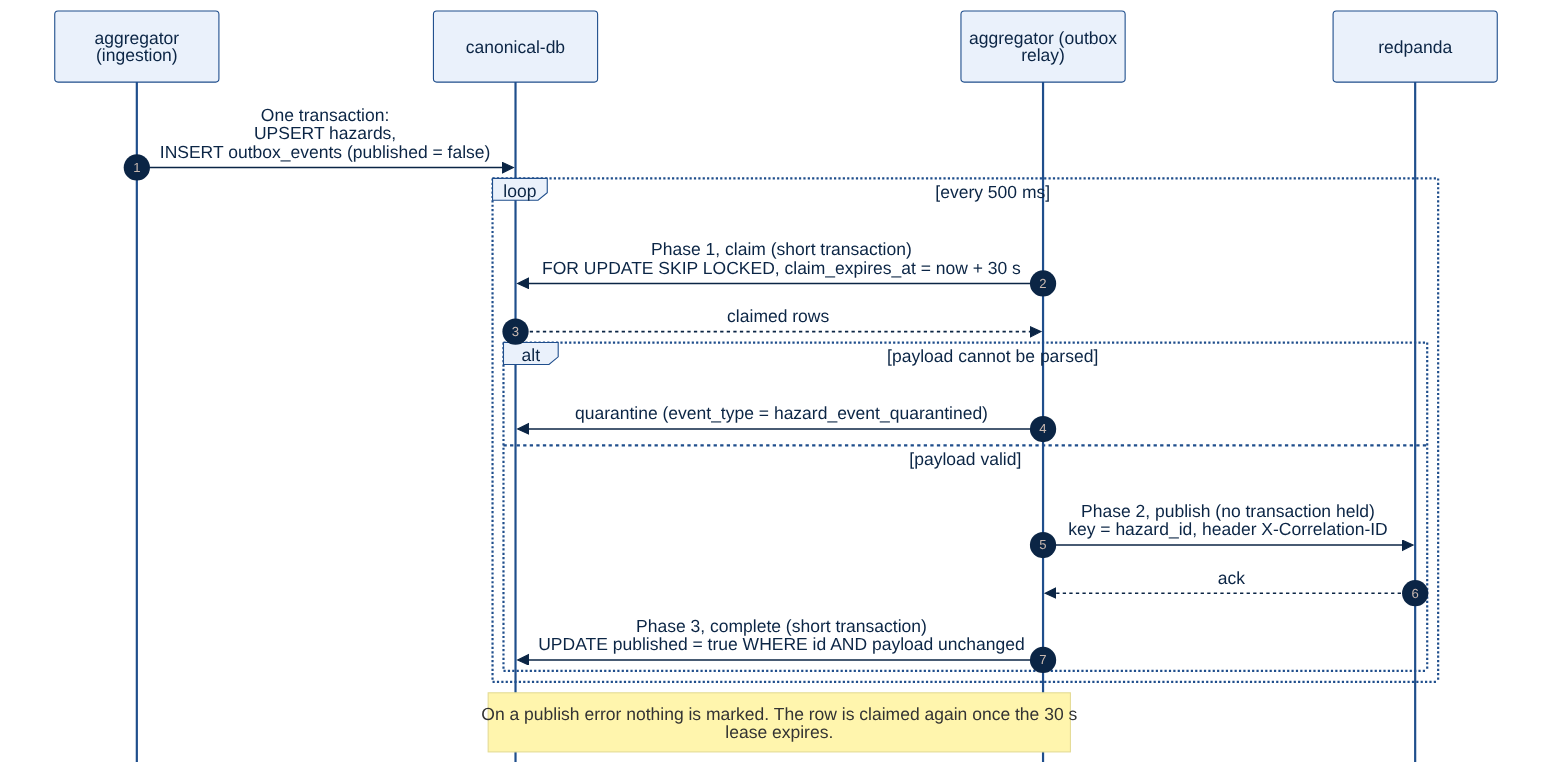
\includegraphics[width=\textwidth,height=0.55\textheight,keepaspectratio]{../diagrams/rendered/adr003-outbox.png}
    \caption[Tiga fase relay Transactional Outbox]{Tiga fase relay Transactional Outbox: claim, publish, dan complete (sumber: \texttt{adr003-outbox.mmd}).}
    \label{fig:relay_outbox}
\end{figure}

\clearpage
\subsection{Alasan Keputusan dan Trade-Off}
Tabel~\ref{tab:storage_eval} menyajikan perbandingan komparatif tiga opsi arsitektur penyimpanan:

\begin{table}[H]
\centering
\footnotesize
\begin{spacing}{1.05}
\caption{Evaluasi Komparatif Alternatif Arsitektur Penyimpanan}
\label{tab:storage_eval}
\begin{tabularx}{\textwidth}{p{2.8cm} X X X}
\toprule
\textbf{Kriteria} & \textbf{PostgreSQL + JSONB (Terpilih)} & \textbf{MongoDB (Document Store)} & \textbf{Strict SQL (EAV / Migrasi DDL)} \\
\midrule
Transaksionalitas \& Pola Outbox & \textbf{Sangat Kuat:} Mendukung transaksi ACID atomik antara tabel \texttt{hazards} dan \texttt{outbox\_events}. & \textbf{Kompleks:} Transaksi \mbox{multi-dokumen} memerlukan replica set (\texttt{--replSet} dan \texttt{rs.initiate()}) sebelum dapat dipakai. & \textbf{Kuat:} Mendukung transaksi ACID penuh. \\
\addlinespace
Agilitas Evolusi Skema & \textbf{Tinggi:} Atribut baru masuk ke JSONB tanpa \textit{table lock} atau migrasi DDL. & \textbf{Tinggi:} Skema dokumen secara alami dinamis. & \textbf{Rendah:} Memerlukan DDL \texttt{ALTER TABLE} atau tabel EAV yang rumit. \\
\addlinespace
Performa Query \& Indexing & \textbf{Tinggi:} Kolom relasional diindeks B-Tree standar; kolom JSONB dapat diindeks GIN. & \textbf{Sedang:} Kueri dokumen sangat cepat, namun tidak mendukung relasi JOIN. & \textbf{Sedang--Rendah:} Pola EAV memperlambat kueri karena banyaknya operasi JOIN. \\
\addlinespace
Kompleksitas Operasional & \textbf{Rendah:} Satu mesin basis data melayani kebutuhan relasional dan dokumen fleksibel. & \textbf{Sedang:} Menambah langkah inisialisasi replica set pada saat \textit{startup}. & \textbf{Rendah:} Mesin relasional tunggal namun beban migrasi skema tinggi. \\
\bottomrule
\end{tabularx}
\end{spacing}
\end{table}

\subsection{Batasan yang Disadari}
\begin{itemize}
    \item Kolom JSONB tidak menegakkan validasi tipe data pada level basis data. Integritas tipe nilai dalam atribut dinamis sepenuhnya menjadi tanggung jawab lapisan kode normalizer di Aggregator.
    \item Kueri berbasis teks bebas atau pencarian parsial di dalam dokumen \mbox{JSONB} yang belum diindeks GIN memerlukan \textit{full-table scan} parsial jika tabel bertumbuh hingga jutaan baris.
\end{itemize}

\subsection{Bukti Penyelesaian}
Verifikasi empiris diotomasi via target \texttt{make demo-p4} (\path{scripts/test_storage_restart.sh}) dengan rekaman log tersimpan pada berkas \path{docs/evidence/p4/storage_restart.log}:
\begin{enumerate}
    \item \textbf{Koeksistensi Skema Heterogen pada PostgreSQL (P4-02):}
    Kueri langsung ke basis data \texttt{canonical-db} membuktikan koeksistensi record sebelum dan setelah evolusi skema:

\noindent\begin{minipage}{\linewidth}
\begin{lstlisting}[language=SQL, caption={Hasil Kueri PostgreSQL Menunjukkan Koeksistensi Atribut Heterogen}]
-- Kueri LIMIT 3 pada tabel hazards (cuplikan, dipangkas)
-- BMKG  SEISMIC  WASPADA: {"depth_km": 37, "magnitude": 5, "potential_tsunami": false}
-- BMKG  SEISMIC  NORMAL : {"depth_km": 36, "magnitude": 4.9, "potential_tsunami": true}
-- PVMBG VOLCANIC WASPADA: {"volcano_id": "VLC-002", "confidence_level": 0.82,
--                          "eruption_count_24h": 8, "ash_column_height_m": 350}
\end{lstlisting}
\end{minipage}

    \item \textbf{Uji Restart Kontainer Independen (P4-01):}
    Kontainer \texttt{aggregator} dijalankan ulang (\textit{restart}) via Docker Compose. Selama proses berjalan, \texttt{client-api} (:8080) dan \textit{mock services} tetap merespons dengan HTTP 200 tanpa mengalami kegagalan berantai.
    \item \textbf{Pemulihan Mandiri Sambungan Basis Data:}
    Kontainer \texttt{canonical-db} dijalankan ulang (\textit{restart}). Klien API mendeteksi ketiadaan basis data sementara dan seketika pulih melayani permintaan dengan HTTP 200 begitu PostgreSQL siap menerima koneksi kembali.
\end{enumerate}

\subsection{Jawaban Butir Spesifikasi (Di Laporan)}
\textbf{Pertanyaan:} \textit{Jelaskan alasan penentuan batas tiap service, mengapa dipecah seperti itu dan bukan dengan pembagian lain. Serta, bandingkan minimal dua alternatif penyimpanan beserta konsekuensi dari pilihan yang diambil.}

\textbf{Jawaban:}
\begin{enumerate}
    \item \textbf{Alasan Penentuan Batas Service (\textit{Service Boundaries}):}
    Service dipecah berdasarkan batas domain dan tingkat perubahan (\textit{rate of change}):
    \begin{itemize}
        \item \textit{Aggregator} dipisahkan karena memiliki dependensi polling aktif dan merupakan satu-satunya penulis (\textit{single writer}) ke penyimpanan kanonis.
        \item \textit{Client-API} dipisahkan agar dapat diskalakan secara horizontal sesuai lonjakan lalu lintas baca publik tanpa membebani thread penarik data ke hulu.
        \item \textit{Auth Service} dipisahkan guna mengisolasi rahasia tanda tangan token kriptografi serta mencegah beban verifikasi autentikasi mengganggu pipa ingesti darurat.
    \end{itemize}
    \item \textbf{Perbandingan Alternatif Penyimpanan:}
    Dua alternatif utama dievaluasi (Tabel~\ref{tab:storage_eval}):
    \begin{itemize}
        \item \textit{Alternatif 1: Basis Data Dokumen Murni (MongoDB):} Keuntungannya fleksibel secara alami, namun konsekuensi buruknya adalah implementasi Transactional Outbox memerlukan transaksi \mbox{multi-dokumen}, yang pada MongoDB hanya tersedia pada replica set. Pengujian pada \texttt{mongo:7.0} menunjukkan mongod \textit{standalone} menolak transaksi, sedangkan replica set satu anggota sudah cukup, tetapi langkah \texttt{rs.initiate()} harus dijalankan lebih dahulu sebelum aplikasi dapat menulis (lihat ADR 003).
        \item \textit{Pilihan Terpilih: PostgreSQL 16 dengan Kolom JSONB:} Konsekuensinya adalah kelompok harus menjaga validasi skema atribut dinamis di lapisan aplikasi, namun memperoleh keuntungan besar berupa transaksi ACID tunggal atomik untuk outbox event, pengindeksan relasional yang matang, serta keandalan operasional tingkat tinggi.
    \end{itemize}
\end{enumerate}

\clearpage
\section{Problem 5: Fan-out Event Distribution atau Publish--Subscribe}
\label{sec:solusi_p5}

\subsection{Rancangan Solusi dan Mekanisme}
\label{subsec:p5_rancangan}
Pada sistem agregasi bencana multi-lembaga, ragam pemangku kepentingan hilir terus bertambah seiring waktu (pembaruan metrik visual pada \textit{dashboard}, pengiriman notifikasi darurat ke tim lapangan, serta portal pemda eksternal).

Apabila \textit{Aggregator Service} memanggil seluruh sistem hilir secara sinkron melalui HTTP/REST langsung (\textit{point-to-point synchronous chaining}), muncul permasalahan \textit{cascading latency} dan \textit{tight coupling}: keterlambatan pada satu konsumen akan menahan siklus eksekusi \textit{Aggregator} dan menunda pengiriman data ke konsumen lain yang mendesak, serta penambahan konsumen baru mewajibkan modifikasi kode dan \textit{redeploy}.

Untuk mengatasi permasalahan tersebut, perancangan sistem menerapkan pola arsitektur \textbf{\textit{Publish--Subscribe}} berbasis \textit{log-based message broker} menggunakan Redpanda (kompatibel penuh dengan protokol Apache Kafka). Rancangan dan mekanisme solusi adalah sebagai berikut:
\begin{enumerate}
    \item \textbf{Decoupled Event Publishing:}
    Setelah \textit{Aggregator Service} menerima, memetakan, dan memvalidasi rekaman bencana dari lembaga sumber, \textit{Aggregator} menerbitkan entitas kanonikal \texttt{HazardEvent} ke \textit{topic} \texttt{bnpb.hazard-events} pada Redpanda. \textit{Topic} ini dikonfigurasi dengan 3 partisi dan memanfaatkan \texttt{hazard\_id} sebagai \textit{partition key} untuk menjamin \textit{causal ordering} per kejadian bencana. Penerbitan dilakukan secara asinkron tanpa keterikatan terhadap identitas, alamat IP, maupun ketersediaan konsumen mana pun.
    \item \textbf{Independent Consumer Groups:}
    Setiap layanan konsumen hilir beroperasi di bawah \textit{consumer group} yang terisolasi secara independen:
    \begin{itemize}
        \item \texttt{bnpb-dashboard-group}: Dikelola oleh \textit{Dashboard Consumer} untuk agregasi metrik frekuensi dan keparahan bencana.
        \item \texttt{bnpb-notifier-group}: Dikelola oleh \textit{Notifier Consumer} untuk mengirimkan notifikasi simulasi peringatan tingkat \textit{Waspada}, \textit{Siaga}, dan \textit{Awas}.
        \item \texttt{bnpb-evaluator-audit-group} / Konsumen Eksternal: Konsumen ketiga (misalnya audit atau portal pemda) yang dapat mendaftar dan membaca aliran data secara independen.
    \end{itemize}
    Masing-masing kelompok konsumen mengelola posisi penunjuk pembacaan (\textit{committed offset}) secara terpisah pada metadata Redpanda (\texttt{\_\_consumer\_offsets}). Kecepatan konsumsi maupun gangguan pada satu grup tidak berdampak sama sekali terhadap grup lainnya.
    \pagebreak
    \item \textbf{Consumer Downtime Resilience dan Backlog Recovery:}
    Apabila suatu layanan konsumen (misalnya \textit{Dashboard}) mengalami kegagalan proses atau dihentikan (\textit{downtime}), Redpanda tetap menyimpan pesan-pesan baru yang diterbitkan produser ke dalam \textit{append-only log} pada disk broker. Nilai \textit{consumer lag} untuk grup tersebut akan bertambah secara proporsional. Sementara itu, konsumen lain (\textit{Notifier}) tetap memproses pesan baru secara \textit{real-time} tanpa terganggu. Ketika layanan yang mati dihidupkan kembali, konsumen membaca ulang konfigurasi \textit{committed offset} terakhirnya dan segera mengejar ketertinggalan (\textit{catch-up backlog}) hingga nilai \textit{lag} kembali ke nol.
    \item \textbf{Manual Offset Commit Discipline:}
    Konsumen mengimplementasikan pustaka \texttt{kafka-go} dengan pembacaan berbasis \texttt{FetchMessage}. \textit{Offset} pesan tidak dikomit secara otomatis, melainkan secara manual melalui \texttt{CommitMessages} tepat setelah pemrosesan data internal dan deduplikasi lokal berhasil diselesaikan. Hal ini menjamin semantik pengiriman \textit{at-least-once}.
\end{enumerate}

\subsection{Alasan Keputusan dan Trade-Off}
\label{subsec:p5_alasan}
Pemilihan pola dan teknologi distribusi \textit{event} didasarkan pada perbandingan arsitektur berikut:

\begin{enumerate}
    \item \textbf{Pola Publish--Subscribe vs. Pola Polling Sinkron / Webhook:}
    \begin{itemize}
        \item \textit{Polling Terjadwal:} Jika konsumen secara berkala melakukan \mbox{HTTP} GET ke \textit{Aggregator}, timbul beban kueri basis data berulang (\textit{database thrashing}) dan latensi deteksi bencana menjadi tinggi tergantung interval \textit{polling}.
        \item \textit{Direct Webhook/HTTP Calls:} Membebani \textit{Aggregator} dengan tanggung jawab \textit{retry}, manajemen kegagalan koneksi, \textit{timeout handling}, dan registrasi dinamis URL konsumen.
        \item \textit{Keputusan:} Pola \textit{Publish--Subscribe} dipilih karena memisahkan tanggung jawab secara bersih (\textit{separation of concerns}). Produser berfokus pada validasi dan penerbitan \textit{event}, sedangkan broker menangani retensi, \textit{buffering}, partisi, dan distribusi data.
    \end{itemize}
    \item \textbf{Pemilihan Redpanda (Log-based Pub/Sub) vs. Tradisional Message Queue (RabbitMQ AMQP):}
    \begin{itemize}
        \item \textit{RabbitMQ (AMQP Fanout Exchange):} Menyediakan mekanisme distribusi pesan yang baik, namun model antreannya menghapus pesan setelah diakui (\textit{destructive read}). Apabila konsumen baru mendaftar di kemudian hari atau konsumen yang mati membutuhkan pemutaran ulang (\textit{replayability}) dari \textit{offset} awal hari, antrean AMQP membutuhkan konfigurasi antrean terpisah sebelum pesan diterbitkan.
        \item \textit{Redpanda (Kafka API):} Menggunakan model \textit{immutable distributed commit log}. Pesan dipertahankan berdasarkan durasi retensi waktu dan kuota penyimpanan fisik, bukan status pembacaan konsumen. Konsumen baru dapat bergabung kapan saja dan membaca data tanpa intervensi produser. Redpanda dipilih karena diimplementasikan dalam C++ tanpa ketergantungan JVM atau Zookeeper, dan kompatibel dengan API Kafka. Hemat memori bukan alasan pemilihan: saat idle, Redpanda (352 MiB) tidak lebih ringan daripada Kafka 3.7 mode KRaft (297 MiB; lihat ADR 002).
    \end{itemize}
\end{enumerate}

\clearpage
\noindent\textbf{Trade-Off Arsitektural:}
\begin{itemize}
    \item \textbf{Kelebihan:} Produser tidak bergantung pada identitas atau ketersediaan konsumen; broker mengisolasi gangguan komponen hilir (\textit{fault isolation}); dan konsumen baru dapat ditambahkan tanpa mengubah produser.
    \item \textbf{Konsekuensi Negatif:} Diperlukan pengelolaan infrastruktur broker pesan tambahan (\textit{cluster health}, partisi, dan kuota disk); data pada sistem hilir bersifat \textit{eventually consistent} dan dapat tertunda ketika terdapat backlog; konsumen wajib menangani potensi duplikasi pesan akibat semantik \textit{at-least-once}. Latensi \textit{fan-out} belum diukur secara khusus pada Milestone 1.
\end{itemize}

\subsection{Batasan yang Disadari}
\label{subsec:p5_batasan}
Batasan teknis yang disadari dan sengaja dibatasi pada lingkup implementasi saat ini meliputi:
\begin{enumerate}
    \item \textbf{Deduplikasi Dalam Memori Bersifat Ephemeral:}
    Pada implementasi prototipe \textit{Dashboard} dan \textit{Notifier}, deduplikasi \texttt{hazard\_id} disimpan dalam struktur \textit{hash map} berbasis memori (\texttt{sync.Mutex} di Go). Apabila kontainer konsumen dihentikan secara paksa atau di-\textit{restart}, riwayat kunci deduplikasi dalam memori akan tereset.
    \item \textbf{Edge Case At-Least-Once pada Crash Antara Eksekusi dan Commit:}
    Apabila konsumen mengalami kegagalan sistem (\textit{panic} atau \textit{SIGKILL}) tepat setelah efek samping dijalankan (misalnya mencetak log agregasi) tetapi sebelum fungsi \texttt{reader.CommitMessages()} dieksekusi, pesan yang sama akan dikonsumsi kembali setelah kontainer hidup kembali.
    \item \textbf{Batas Retensi Log Broker:}
    Penyimpanan pesan pada Redpanda dibatasi oleh kebijakan retensi waktu dan ukuran log. Jika konsumen mengalami \textit{downtime} melebihi durasi retensi log yang dikonfigurasi, pesan-pesan terlama yang belum terbaca akan terhapus secara otomatis oleh broker sehingga konsumen tidak dapat lagi memulihkan data tersebut secara utuh.
\end{enumerate}

\clearpage
\subsection{Bukti Penyelesaian}
\label{subsec:p5_bukti}
Pengujian dan validasi solusi Problem 5 dilakukan secara otomatis melalui skrip \path{scripts/test_consumer_recovery.sh} (dapat dijalankan melalui \texttt{make demo-p5}). Seluruh pengujian mencakup verifikasi partisi, penerbitan paralel, pemulihan \textit{downtime}, dan penambahan konsumen dinamis.

\noindent\begin{minipage}{\linewidth}
\begin{lstlisting}[language=bash, caption={Keluaran Eksekusi Pengujian Otomatis Problem 5 (Fan-Out \& Downtime Recovery)}]
[Step 0] Checking Redpanda topic: 'bnpb.hazard-events' (3 partitions) -> [PASS]
[Step 1] Starting Dashboard and Notifier containers -> [PASS]
[Step 2] Publishing event 'c08-fanout-...' -> Fan-out received by both -> [PASS]
[Step 3] Stopping Dashboard and publishing recovery event during downtime:
GROUP                 TOPIC               STATUS    TOTAL-LAG
bnpb-dashboard-group  bnpb.hazard-events  Empty     1
[PASS] Notifier processed; Dashboard offline and accumulated TOTAL-LAG = 1
[Step 4] Restarting Dashboard and verifying backlog recovery:
GROUP                 TOPIC               STATUS    TOTAL-LAG
bnpb-dashboard-group  bnpb.hazard-events  Stable    0
[PASS] Dashboard resumed committed offset; TOTAL-LAG returned to zero
[Step 5] Dynamic 3rd consumer joined -> Events received -> [PASS]
Results: 11 passed, 0 failed. Fan-Out & Recovery Verified!
\end{lstlisting}
\end{minipage}

\noindent\textbf{Analisis Bukti Log:}
\begin{enumerate}
    \item \textbf{Fan-Out Verifikasi (Langkah 2):} Satu kejadian bencana (\texttt{c08-fanout-...}) diterbitkan ke Redpanda. Kedua layanan (\textit{Dashboard} dan \textit{Notifier}) mendeteksi dan memproses pesan tersebut secara simultan dalam kelompok konsumen masing-masing (\texttt{bnpb-}\allowbreak\texttt{dashboard-}\allowbreak\texttt{group} dan \texttt{bnpb-}\allowbreak\texttt{notifier-}\allowbreak\texttt{group}).
    \item \textbf{Downtime \& Lag Accumulation (Langkah 3):} Saat kontainer \textit{Dashboard} dimatikan paksa, pengiriman event baru (\texttt{c08-recovery-...}) tetap diproses normal oleh \textit{Notifier}. Pemeriksaan Redpanda via \texttt{rpk group describe} menunjukkan \texttt{TOTAL-LAG = 1} pada \textit{Dashboard}, membuktikan pesan aman tersimpan pada broker dan tidak hilang.
    \item \textbf{Backlog Catch-Up (Langkah 4):} Begitu kontainer \textit{Dashboard} dinyalakan kembali, konsumen segera menyerap pesan yang tertinggal dan melakukan \textit{manual commit}, ditandai dengan \texttt{TOTAL-LAG} yang kembali menjadi 0.
    \item \textbf{Penambahan Konsumen Baru (Langkah 5):} Kontainer independen ketiga (\texttt{bnpb-}\allowbreak\texttt{evaluator-}\allowbreak\texttt{audit-...}) dijalankan pada topik \texttt{bnpb.hazard-events} tanpa melakukan \textit{restart} atau pengubahan kode apa pun pada \textit{Aggregator Service}. Konsumen baru langsung menerima \textit{event} secara transparan.
\end{enumerate}

\clearpage
\subsection{Jawaban Butir ``Di Laporan''}
\label{subsec:p5_jawaban}
Jawaban komprehensif atas aspek evaluasi Problem 5:

\begin{enumerate}
    \item \textbf{Broker dan Pola yang Dipilih:}
    \begin{itemize}
        \item \textbf{Broker (Redpanda):} Kompatibel API Kafka v3, arsitektur \textit{single binary} C++ (tanpa JVM dan ZooKeeper), serta dukungan utilitas CLI \texttt{rpk}.
        \item \textbf{Pola (Pub--Sub Log Terdistribusi):} Topik \texttt{bnpb.hazard-events} dibagi ke 3 partisi dengan \textit{consumer groups} mandiri untuk replikasi aliran pesan (\textit{fan-out}) ke setiap grup secara otonom.
    \end{itemize}

    \item \textbf{Semantik Pengiriman yang Berlaku (\textit{At-Least-Once Delivery}):}
    \begin{itemize}
        \item Produser (outbox relay pada Aggregator) mengirimkan pesan dengan tingkat pengakuan \texttt{acks=1} (\texttt{kafka.RequireOne}), sehingga pesan telah dicatat oleh \textit{leader} partisi sebelum dianggap sukses.
        \item Konsumen tidak memakai komit otomatis: pesan dibaca via \texttt{reader.FetchMessage}, lalu memanggil \texttt{reader.CommitMessages} secara manual tepat setelah pemrosesan dan deduplikasi selesai.
        \item Jika terjadi kegagalan jaringan atau proses mati sebelum komit, \textit{offset} belum tersimpan sehingga pesan dapat dikirim ulang (\textit{redeliver}) saat pulih. Kombinasi transactional outbox, retry, retensi broker, dan komit manual mendukung semantik \textit{at-least-once} selama basis data dan log broker tetap tersedia; rancangan single-node dengan \texttt{acks=1} bukan jaminan absolut \textit{zero message loss}.
    \end{itemize}

    \item \textbf{Konsekuensi bagi Consumer dan Perlunya Sifat Idempoten:}
    \begin{itemize}
        \item \textbf{Kebutuhan Idempotensi:} Dalam semantik \textit{at-least-once}, pengiriman ganda (\textit{duplicate delivery}) dapat terjadi saat \textit{timeout}, retry, atau partisi \textit{rebalance}. Tanpa idempotensi, metrik bencana dapat terhitung ganda (\textit{double count}) pada Dashboard dan memicu notifikasi berulang (\textit{alert fatigue}) pada Notifier.
        \item \textbf{Strategi Mitigasi (\textit{Event Identity}):} Setiap bencana membawa identitas global deterministik (\texttt{hazard\_id}). Pada prototipe saat ini, konsumen mengelola set \texttt{processed[hazard\_id]} dalam memori dengan perlindungan \texttt{sync.Mutex} untuk mengabaikan duplikasi sebelum komit. Pada skala multi-replika produksi, hal ini disikapi via operasi atomik (Redis \texttt{SETNX}) atau integritas basis data relasional (\texttt{ON CONFLICT DO NOTHING}).
    \end{itemize}
\end{enumerate}


% Bab 4: Petunjuk Menjalankan Sistem
\chapter{Petunjuk Menjalankan Sistem}
\label{chap:petunjuk}

Bab ini menyajikan panduan ringkas operasional untuk mengonfigurasi, menjalankan, dan memverifikasi seluruh komponen \textit{Disaster Data Aggregator Platform} pada lingkungan pengujian evaluator. Panduan lengkap dan komprehensif didokumentasikan pada berkas \texttt{README.md} di direktori utama repositori.

\section{Prasyarat dan Konfigurasi Lingkungan}
\label{sec:petunjuk_prasyarat}

Sebelum menjalankan sistem, pastikan perangkat kerja penguji telah memenuhi kebutuhan piranti lunak berikut:
\begin{enumerate}
    \item \textbf{Docker Engine \& Docker Compose:} Docker Engine minimal versi 24.0+ dan Docker Compose Plugin minimal versi v2.20+.
    \item \textbf{Go Toolchain (Opsional untuk kompilasi lokal):} Go v1.22+ (seluruh layanan telah memiliki kontainerisasi terisolasi sehingga instalasi Go lokal bersifat opsional).
    \item \textbf{Utilitas Terminal:} \texttt{make}, \texttt{curl}, \texttt{jq}, dan \texttt{bash} untuk mengeksekusi skrip otomatisasi.
    \item \textbf{Alat Pengujian Beban (Opsional):} \texttt{k6} (jika tidak terpasang di \textit{host}, target pengujian \texttt{make load-test} akan secara otomatis mengunduh dan menjalankan citra kontainer \texttt{grafana/k6}).
\end{enumerate}

\noindent\textbf{Langkah Konfigurasi Lingkungan (\textit{Environment Setup}):}
\begin{lstlisting}[language=bash, caption={Inisialisasi Variabel Lingkungan}]
# Salin template variabel lingkungan dari .env.example
cp .env.example .env

# (Opsional) Sesuaikan nilai rahasia atau port jika diperlukan
\end{lstlisting}

\section{Langkah Menjalankan Sistem}
\label{sec:petunjuk_menjalankan}

Seluruh orkestrasi kontainer (\textit{mock services}, basis data, broker Redpanda, layanan inti BNPB, dan konsumen hilir) dikelola melalui \texttt{Makefile} dan \texttt{docker-compose.yml}:

\begin{enumerate}
    \item \textbf{Menjalankan Seluruh Platform:}
    Eksekusi perintah berikut untuk membangun citra kontainer dan mengaktifkan 11 kontainer layanan di latar belakang:
    \begin{lstlisting}[language=bash]
make up
# Ekuivalen dengan: docker compose up -d --build
    \end{lstlisting}
    Tunggu sekitar 5--10 detik hingga kontainer \texttt{redpanda-init} selesai menginisialisasi partisi dan seluruh layanan berstatus \textit{healthy}.

    \item \textbf{Verifikasi Status Kesehatan Layanan (\textit{Health Checks}):}
    Pastikan seluruh titik akhir publik dan internal merespons dengan status \texttt{"UP"}:
    \begin{lstlisting}[language=bash]
curl -s http://localhost:8081/health | jq .   # mock-bmkg
curl -s http://localhost:8082/health | jq .   # mock-pvmbg
curl -s http://localhost:8084/health | jq .   # auth service
curl -s http://localhost:8080/health | jq .   # client-api gateway
docker compose exec client-api curl -s http://aggregator:8083/health | jq . # aggregator
    \end{lstlisting}

    \item \textbf{Melihat Log Layanan Secara Kolektif:}
    \begin{lstlisting}[language=bash]
make logs
    \end{lstlisting}

    \item \textbf{Menghentikan Sistem dan Membersihkan Lingkungan:}
    \begin{lstlisting}[language=bash]
make down
# Ekuivalen dengan: docker compose down -v
    \end{lstlisting}
\end{enumerate}

\section{Langkah Verifikasi dan Demonstrasi Solusi (Problem 1--5)}
\label{sec:petunjuk_verifikasi}

Repositori menyediakan target otomatisasi \texttt{make} terintegrasi untuk mereplikasi dan memvalidasi kriteria evaluasi setiap permasalahan:

\begin{table}[htbp]
\centering
\small
\caption{Matriks Verifikasi dan Target Eksekusi Demonstrasi Permasalahan}
\label{tab:runbook_matrix}
\begin{tabularx}{\textwidth}{@{}l l l X@{}}
\toprule
\textbf{Problem} & \textbf{Target Make} & \textbf{Skrip Pengujian} & \textbf{Kriteria Utama yang Diverifikasi} \\
\midrule
\textbf{Problem 1} & \texttt{make demo-p1} & \texttt{scripts/test\_schema\_change.sh} & Evolusi skema aditif (\texttt{confidence\_level}) diserap dinamis tanpa migrasi database atau \textit{redeploy}. \\
\addlinespace
\textbf{Problem 2} & \texttt{make demo-p2} & \texttt{scripts/test\_outage.sh} & Simulasi pemadaman PVMBG; respons terdegradasi (\texttt{degraded: true}); BMKG tetap normal. \\
& \texttt{make load-test} & \texttt{scripts/load\_test.js} & Uji beban 50 koneksi konstan selama 60 detik (k6) dengan tingkat keberhasilan 100\%. \\
\addlinespace
\textbf{Problem 3} & \texttt{make demo-p3} & \texttt{scripts/test\_cross\_credential.sh} & Isolasi \textit{trust domain} upstream (penolakan kredensial silang BMKG/PVMBG). \\
& & \texttt{scripts/test\_auth\_scopes.sh} & Penolakan akses \texttt{403} bagi Media pada \textit{raw fields}; rotasi penyegaran token JWT (TTL 60 detik). \\
\addlinespace
\textbf{Problem 4} & \texttt{make demo-p4} & \texttt{scripts/test\_storage\_restart.sh} & \textit{Independent container rebuild} dan \textit{restart}; isolasi kegagalan tanpa efek kaskade ke basis data. \\
\addlinespace
\textbf{Problem 5} & \texttt{make demo-p5} & \texttt{scripts/test\_consumer\_recovery.sh} & Distribusi \textit{fan-out}; akumulasi \textit{lag} saat \textit{consumer downtime}; pemulihan \textit{offset}; penambahan konsumen ke-3. \\
\bottomrule
\end{tabularx}
\end{table}

\noindent Setiap berkas log lengkap hasil demonstrasi pengujian otomatis ini juga diarsipkan pada direktori repositori \texttt{docs/evidence/p1/} hingga \texttt{docs/evidence/p5/}.


% Daftar Pustaka
\newpage
\addcontentsline{toc}{chapter}{Daftar Pustaka}
\bibliographystyle{plainnat}
\bibliography{references}

% Lampiran
\appendix
\chapter{Pernyataan Penggunaan Kecerdasan Buatan (AI)}
\label{chap:ai_declaration}

Sesuai dengan ketentuan penulisan pada dokumen spesifikasi tugas besar IF4031 Arsitektur Aplikasi Terdistribusi (Milestone 1), tim pengembang mendeklarasikan secara terbuka dan jujur penggunaan model bahasa besar (\textit{Large Language Model} / AI) selama proses perancangan, implementasi, dan penyusunan laporan.

\section*{Deklarasi Penggunaan}
Tim pengembang memanfaatkan alat bantu AI (\textit{Antigravity CLI}, \textit{Anthropic Claude}, dan \textit{OpenAI ChatGPT}) untuk keperluan:
\begin{enumerate}
    \item \textbf{Eksplorasi Sintaksis dan \textit{Boilerplate}:} Pembuatan kerangka awal sintaks Go (seperti struktur pengurai JSON dan konfigurasi pustaka \texttt{kafka-go}) serta template skrip pengujian Bash dan k6.
    \item \textbf{\textit{Proofreading} dan Penyempurnaan Tata Bahasa:} Pemeriksaan konsistensi istilah teknis, keterbacaan kalimat, dan format penataan dokumen LaTeX.
    \item \textbf{Perumusan Alternatif Arsitektural:} Diskusi mengenai perbandingan kelebihan dan kelemahan pola \textit{Transactional Outbox} serta pertimbangan trade-off antara PostgreSQL JSONB dan MongoDB.
\end{enumerate}

\section*{Pernyataan Tanggung Jawab dan Pemahaman}
Seluruh anggota kelompok menyatakan dengan sesungguhnya bahwa:
\begin{enumerate}
    \item Seluruh keputusan arsitektur, pemilihan teknologi, pembagian batas layanan (\textit{bounded context}), dan logika bisnis inti dirumuskan, didiskusikan, dan diputuskan secara mandiri oleh tim pengembang.
    \item Seluruh kode yang dihasilkan atau disempurnakan oleh alat bantu AI telah dibaca, ditelaah, dipahami sepenuhnya, serta diuji validitas dan fungsionalitasnya oleh anggota kelompok penanggung jawab komponen terkait.
    \item Seluruh isi laporan ini merepresentasikan pekerjaan orisinal kelompok. Tim pengembang bertanggung jawab penuh atas kebenaran, integritas akademik, dan keandalan sistem yang diajukan.
\end{enumerate}

\vspace{1.5cm}

\begin{table}[htbp]
\centering
\begin{tabularx}{\textwidth}{X X X}
Bandung, 8 Oktober 2026 & Bandung, 8 Oktober 2026 & Bandung, 8 Oktober 2026 \\
\vspace{1.5cm} & \vspace{1.5cm} & \vspace{1.5cm} \\
\textbf{Aldoy Fauzan Avanza} & \textbf{Darrel Adinarya Sunanda} & \textbf{Jennifer Khang} \\
NIM: 18223113 & NIM: 13523061 & NIM: 13524110 \\
\end{tabularx}
\end{table}


\end{document}
